\section{ASTERISK}
A ferramenta de código aberto Asterisk desenvolvida pela Digium, disponibiliza as principais funcionalidades que um \textit{Call Center} necessita, dentre elas a criação de Ramais, Troncos, Rotas, configuração Plano de Discagens, Gravação de Voz, Conferência, Filas, Unidade de Resposta Audível entre diversos outros recursos que podem ser explorados e utilizados, podendo ser utilizado como um PABX IP, assim como se integrado a soluções VoIP ou a rede de telefonia pública.
Com tantos recursos disponíveis a ferramenta Asterisk está muito bem preparada para atender as expectativas, principalmente pelo fato de disponibilizar protocolos de comunicação com sistemas externos, por exemplo, o protocolo AGI (\textit{Asterisk Gateway Interface}), permite o consumo de recursos externos ao Asterisk, já o protocolo AMI (\textit{Asterisk Manager Interface}) permite que aplicações externas enviem ordens para serem executadas no Asterisk, dessa forma a solução pode ser muito bem integrada a sistemas legados.


\subsection{\textbf{Asterisk Conceitos}}

A ferramenta tem como base o Plano de Discagem, sendo ele responsável em definir o que deve acontecer, seja no momento em que for recepcionada uma ligação ou quando for digitado algum número. No plano de discagem podemos definir separações lógicas denominadas contextos\label{key:contexto}, responsáveis em definir um comportamento utilizando os recursos nativos para determinar as instruções (extensões), por exemplo, podemos criar um contexto para definir o que deve acontecer ao receber ligações da rede pública e outro para definir o comportamento para as ligações advindas de ramais internos:

\begin{flushleft}

\textbf{[PSTN]} \\
\textit{exten => 2000,1,Answer();} \\
Contexto chamado “PSTN”, utiliza a extensão 2000, com prioridade 1 e aplicação \textit{Answer}.\\

\textbf{[RAMAIS\_INTERNOS]} \\
exten => 2001,1, Playback(AVISO\_GERAL); \\
Contexto chamado “RAMAIS\_INTERNOS”, utiliza a extensão 2001, com prioridade 1 e aplicação Playback para tocar o áudio AVISO\_GERAL.\\
\end{flushleft}

O número 2000 no contexto “PSTN” utilizado na extensão representa o número informado pelo Originador da chamada, a prioridade trata-se de um parâmetro que representa a ordem de execução das aplicações, normalmente descritos de forma sequencial, já as aplicações são utilizadas para realizar uma ação qualquer. Em cada extensão (exten), podemos utilizar recursos de aplicativos nativos da ferramenta, sejam eles para atender, desligar, gravar o áudio entre outros recursos, dessa forma podemos definir o comportamento para o contexto, assim como realizar a transferência para outros contextos.


\subsection{\textbf{Asterisk Instalação}}

A instalação do Asterisk muita das vezes é uma tarefa cansativa e exige bastante atenção, pois a configuração deve ser realizada em arquivos de texto em uma sintaxe estabelecida pela ferramenta, atualmente existem diversas soluções que fornecem uma interface gráfica para tornar esse processo mais intuitivo e prático, neste trabalho foi utilizada uma distribuição chamada Disc-OS na versão 2.0, que disponibiliza uma interface web para realizar a configuração do Asterisk 1.4, para realizar o processo de instalação do Disc-OS, foram seguidos os passos descritos por Jilsimaico Darú \cite{DARU:2008}, após a realização dos procedimentos, ao iniciar a distribuição Disc-OS automaticamente é iniciado o serviço do Asterisk, dessa forma para acessar o sistema basta digitar no navegador o endereço IP do terminal que está executando o sistema, visualizando a página conforme a figura \ref{figura:asteriskInterfaceWeb} abaixo:


\begin{figure}[H]
	\centering
	\caption{\textbf{Acessando página inicial da Interface WEB do Disc-OS}}	
	\label{figura:asteriskInterfaceWeb}
	\begin{subfigure}[H]{\textwidth}
		\centering
		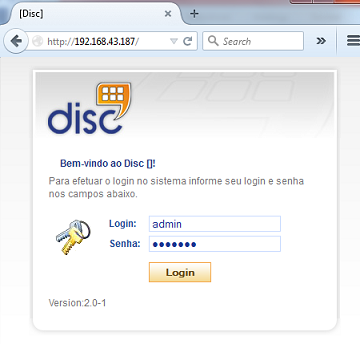
\includegraphics{figuras/pagina_inicial_asterisk.png}
		\legend {\fontsize{10}{12}\selectfont {Fonte: Autoria Própria}.}
	\end{subfigure}
\end{figure}


Para acessar as funcionalidades do sistema basta inserir a seguinte credencial de acesso:\\
\textbf{Login}: admin\\
\textbf{Senha}: disc-os\\


\subsection{\textbf{Asterisk - Detalhamento Técnico}}
A ferramenta de código aberto Asterisk\footnote{Disponível em \url{http://www.asterisk.org}}, tem algumas características importantes e fundamentais para o estudo além de ser uma implementação de uma central telefônica que permite que clientes se comuniquem, tem outros recursos interessantes que fazem da ferramenta uma peça chave no processo da integração proposta, recursos como respostas interativas, correios de voz, realização de conferencias, distribuição automática de chamadas, além de ser flexível a adição de novos recursos tanto por meio de scripts na própria linguagem do Asterisk como também por meio de códigos em linguagem C entre outras formas de customização da ferramenta. Desenvolvido pela empresa Digium sob licença GPL\footnote{GPL - \textit{General Public Lisence}}, atualmente portável em versões Linux, Windows e Mac OS, suportando protocolos de Voz sobre IP (VoIP), assim como SIP e H.323 entre outros. O próprio Asterisk contém um protocolo próprio chamado IAX fornecendo um melhor desempenho entre os entroncamentos entre os servidores Asterisk para casos de maior complexidade.
